% !TEX program = xelatex
\documentclass[conference]{IEEEtran}
\usepackage{cite}
\usepackage{amsmath,amssymb,amsfonts}
\usepackage{algorithmic}
\usepackage{graphicx}
\usepackage{textcomp}
\usepackage{xcolor}
\usepackage{multicol}
%%% For language switching -- like babel, but for xelatex
\usepackage{polyglossia}
%%% For the awesome fontawesome icons!
\usepackage{fontawesome}
\usepackage{multirow}
\usepackage{makecell} % for more vertical space in cells
\setmainlanguage{english}
\setotherlanguages{hindi,sanskrit} %% or other languages

% define fonts for other languages
\newfontfamily\devanagarifont[Script=Devanagari]{Annapurna SIL}

\def\BibTeX{{\rm B\kern-.05em{\sc i\kern-.025em b}\kern-.08em
    T\kern-.1667em\lower.7ex\hbox{E}\kern-.125emX}}

\makeatletter
\newcommand{\linebreakand}{%
  \end{@IEEEauthorhalign}
  \hfill\mbox{}\par
  \mbox{}\hfill\begin{@IEEEauthorhalign}
}
\makeatother
\usepackage{hyperref}
\title{A Rule-based Recursive Lemmatization Algorithm with POS tagging for
  Plagiarism Detection in Nepali texts
% \thanks{Identify applicable funding agency here. If none, delete this.}
}

\author{\IEEEauthorblockN{Ayush Kumar Shah}
  \IEEEauthorblockA{\textit{Department of Computing and Information Sciences} \\
  \textit{Rochester Institute of Technology} \\
Rochester, NY 14623, USA \\
as1211@rit.edu
}}

\begin{document}

\maketitle

\begin{abstract}
There have been many notable works for detecting plagiarism in the English
texts, but none in the Nepali texts, which uses Devanagari scripts. It is mostly
due to the
involved challenges in the pre-processing of Nepali texts caused by the lack of
available datasets and the complicated
grammatical rules and syntactic structure of the Nepali language. Since
pre-processing texts are vital in performing any Natural Language Processing
(NLP) task, we aim to accomplish this task for Nepali texts. The paper
(1) introduces a set of 140 custom suffix and prefix rules to extract the root word, 
that deals with the grammatical complexities and syntactic structure specific to 
the Nepali language, (2) presents a rule-based recursive lemmatization
algorithm, which considers the effect of parts of speech (POS)
to pre-process Nepali texts using these rules, (3) presents a
NEP-PLAG2019v1
dataset\footnote{\url{https://github.com/ayushkumarshah/Nepali_Plagiarism_Detection/tree/master/datasets/NEP-PLAG2019v1}
\\\\Note: The dataset and results of this work have not been generated yet 
and are simply meant to be an exercise in research writing. However, the 
methods and setup are real.}
(4) implements a Nepali Plagiarism Detection System, which uses tf-idf feature vector 
obtained from the pre-processed texts as inputs to compute the Cosine similarity 
to detect plagiarism.
For the NEP-PLAG2019v1 dataset (10,000 pairs), the proposed method was able
to obtain an F1-score of 96.05\%. 
The ability to extract root words with higher accuracy from Nepali texts, 
with the complex grammar and structure handled by the introduced rules, gives
rise to opportunities to perform various NLP tasks in the Nepali language.
\end{abstract}

\begin{IEEEkeywords}
Plagiarism, POS, Tokens, tf-idf, Stemming, Lemmatization
\end{IEEEkeywords}

\section{Introduction}

To identify and deal with plagiarism, we need to 
build a system that can detect
plagiarism of any form in texts. A significant component of such systems
is generating useful features from the texts using appropriate and
accurate stemming or lemmatization algorithm.
There have been many works to address this problem. In 1980, Porter 
presented a simple algorithm\cite{r2} for stemming English language words. 
This algorithm is the basis for pre-processing texts until now. 

Pre-processing of texts written in Devanagari scripts, specifically in the
Nepali language is more challenging than
those in the English language. The general stemmers cannot extract the root word
accurately due to the complex and unique syntactic structure of the Nepali
language. Similarly, the grammatical rules are more vast than in the English
language. For instance, the verbs in the Nepali sentences require gender 
agreement, in addition to the number agreement (in the English language), with 
the subject of the sentence. E.g. the verb "eat" is 
\begin{sanskrit}
  खान्छ  and खान्छे
\end{sanskrit}
for male and female subjects, respectively. 
Likewise, there are different forms of the same pronoun and verb
for different levels of respect for the person. E.g., the sentence "You eat."
becomes
\begin{sanskrit}
तँ  खान्छस् । 
तिमि खान्छौ। 
तपाई खानुहुन्छ।   
\end{sanskrit}
for three different levels of respect for the person.

S.D. Makhija \cite{makhija_study_2016} has described
different types of stemming
algorithms and summarized stemmers designed for different
languages based on Devanagari scripts. D. Monika et.al.
\cite{abhishek_effective_2013} have presented the development of Hindi stemmer
based on Devanagari script for stripping both prefixes and suffixes to obtain
the root word using the combination of lookup algorithm, suffix stripping
algorithm, and prefix removal algorithm. The lookup table approach makes the
system inefficient to use. \cite{dangui_lightweight_2015} used a supervised
approach using n-gram models to design a common stemmer for languages in
Devanagari scripts. They tested four approaches based on frequency,
statistics, length, and iterations to split the words into suffix and stem. This
method does not consider prefix, and the results are worse in the Nepali language,
since the complex grammar and structure specific to the Nepali language are not
considered. \cite{pande_devanagari_nodate} used a unique approach of
romanization (one to one mapping of each vowel and consonant of Devanagari
script into an English roman code to exploit the English coded corpus. The
common limitations in the previous works are not considering the dependency of
stemming on the parts of speech (POS) since the same word occurring as different
POS results, into a different root word, and the different complex grammatical
structures specific to the Nepali language.

This paper aims to overcome the limitations in the previous works by introducing
140 different prefix and suffix rules, which consider the POS and complex
grammar and syntactic structure of the Nepali language to extract the
root words from Nepali texts with higher accuracy. A rule-based recursive
lemmatization algorithm is implemented to pre-process the Nepali texts
effectively using those rules. The paper also contributes a
new dataset NEP-PLAG2019v1 for plagiarism of Nepali texts. Finally, we convert the 
pre-processed tokens into tf-idf feature vectors and compute Cosine similarity measures
between the resulting vectors to classify the pair of texts into Plagiarised and 
Non-Plagiarised classes using a threshold value (25\%). We have obtained an F1-score
of 96.05\% on the NEP-PLAG2019v1 dataset. The
code\footnote{\url{https://github.com/ayushkumarshah/Nepali_Plagiarism_Detection}}
used in our experiments is publicly available.

\section{Preprocessing of documents}
\begin{figure}[htbp]
\centering{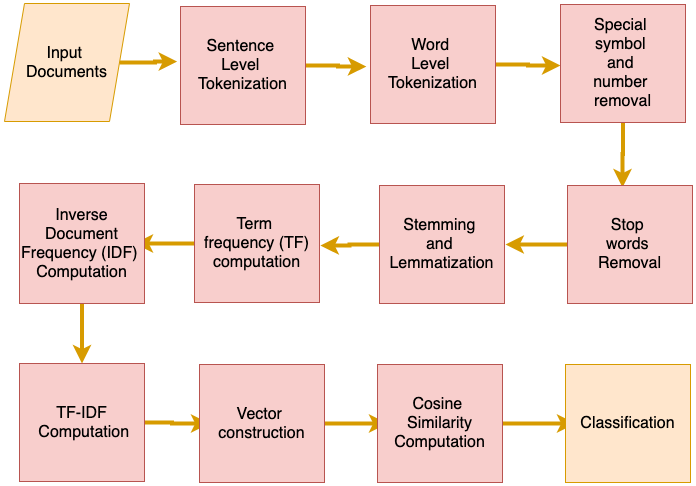
\includegraphics[width=9cm,height=9cm]{figures/flow_diagram.png}} 
\caption{Flow diagram for Plagiarism detection showing the major steps} 
\label{flow} 
\end{figure}
% \begin{figure}[htbp]
% \centering
% 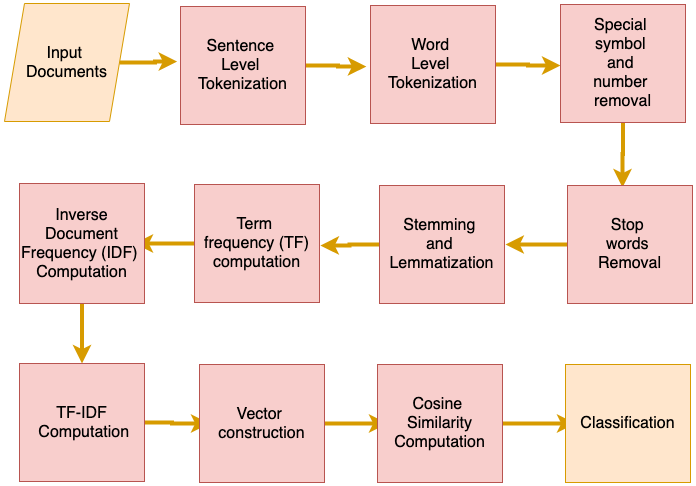
\includegraphics[width=0.525 \textwidth]{figures/flow_diagram.png}
% \caption{Flow diagram for Plagiarism detection showing the major processes
% involved in segmentation and classification}
% \label{fig1}
% \end{figure}

As shown in Figure.~\ref{flow}, there are various operations involved in the
methodology including pre-processing of Devanagari texts using the introduced 
rule-based stemming algorithm, feature vector construction using tf-idf and
finally, similarity computations for the final classifications.

\subsection{Sentence tokenization}

The text in the document is split into sentences, thereby allowing line-by-line
processing in the subsequent sentences. Vertical bars, question marks, and 
exclamation marks are used to break down the text into individual sentences. \\
\\Example:\\\\
\begin{sanskrit}
  "परिश्रम नगरी हुन्छ? परिश्रम सफलताको एक-मात्र बाटो हो। अक्सर जो परिश्रम गर्छ, उही सफल हुन्छ। अब त परिश्रम गर्छौ नि? नगरी कहाँ हुन्छ त!"
\end{sanskrit}\\\\
The following collection of sentences is tokenized into:\\\\
  \begin{sanskrit}
  'परिश्रम नगरी हुन्छ?', 'परिश्रम सफलताको एक-मात्र बाटो हो।', 'अक्सर जो परिश्रम गर्छ, उही सफल हुन्छ।', 'अब त परिश्रम गर्छौ नि?', 'नगरी कहाँ हुन्छ त!'
\end{sanskrit}
\medskip

\subsection{Word tokenization}

The input sentences are broken down into individual tokens. White space and
comma are used to break down the words. \\
\\Example:\\
\begin{sanskrit}
  
['परिश्रम', 'नगरी', 'हुन्छ?', 'परिश्रम', 'सफलताको', 'एक-मात्र', 'बाटो', 'हो।', 'अक्सर', 'जो', 'परिश्रम', 'गर्छ', 'उही', 'सफल', 'हुन्छ।', 'अब', 'त', 'परिश्रम', 'गर्छौ', 'नि?', 'नगरी', 'कहाँ', 'हुन्छ', 'त!']
\end{sanskrit}
\medskip

\subsection {Special symbol and number removal}
Special symbols like ,)({}[]?!।"  "":-- and numbers both in English and Nepali are removed from the tokens using regular expressions.
\medskip

\subsection {Stop words removal}
Stop words are high-frequency words that do not have much influence in the text and are removed to increase the performance.
A list of 592  stop-words like \begin{sanskrit}त्यही, जब, अथवा,\end{sanskrit} were collected, and these words were removed from the list of tokens. 
\medskip

% \renewcommand{\labelenumii}{\roman{enumii}}
\section {Stemming and Lemmatization}

Our primary contribution constitutes the stemming and lemmatization algorithm for
the Nepali language. We have taken POS and complex grammatical and syntactic
structures into account to design the algorithm. Lemmatization is more complex
than stemming since the result of lemmatization is a meaningful word present in
the dictionary as opposed to stemming. We have implemented lemmatization using a
corpus of words in the Nepali dictionary to ensure we almost always get a valid
root word. Hence, the features used to construct vectors are a better representation
of the document, while the irrelevant features are removed. 
We have developed our algorithm with the help of the 
Language Technical Kendra\footnote{\url{http://ltk.org.np/}}. Note that the term
'stemmer' used throughout the paper corresponds to the lemmatization algorithm
although the name suggests a stemming algorithm.

\subsection {Prerequisites of the Stemmer}

The prerequisites of the Stemmer Module would be the
following \cite{r10}:

\begin{enumerate}
  \item POS Tagset
  \item Tokenizer
  \item Free morpheme-based lexicon
  \item Two sets of affixes for the suffix and prefix
  \item A database of word breaking grammatical rules
\end{enumerate}

\subsection {POS Tagset}

The NLP team at Madan Puraskar Pustakalaya,
Nepal has developed a relatively simplified POS
Tagset of 91 tags. The tagset has been developed
targeting the Grammar Checker for Nepali. The tagset
development guidelines and experiences of Hindi,
Urdu and some others like the British National Corpus
have been consulted in developing the current POS
Tagset. The POS tag coverage test of the developed
POS TagSet is currently being tested. For the testing
purpose, the free morpheme list entries and the
affixes list are being POS tagged \cite{r10}.

\subsection {Set of Affixes}

Stemming is a crude heuristic process that chops off the ends of words in the hope of 
achieving root words (morphemes) and often includes the removal of
derivational affixes. There are two sets of affixes: suffixes and prefixes. The prefixes and suffixes
are stemmed for obtaining a root word.

For example, 
In a word \begin{sanskrit} 'सफलताको' 
, 'सफल' \end{sanskrit} is a root and it is combined with the suffix
\begin{sanskrit}‘ता’\end{sanskrit}  and \begin{sanskrit}‘को’\end{sanskrit} and the
resulting form becomes \begin{sanskrit} 'सफलताको'. \end{sanskrit}Some of the prefix
and suffix in the dataset is as follows:\\\\
Prefix set: \qquad Suffix set:\\
\begin{sanskrit}
न|1\hspace{52pt} यो|17\\
उप|2\hspace{50pt}दा|18\\
महा|3\hspace{48pt}दै|19\\
अ|4\hspace{50pt} ँदै|19\\
सु|5\hspace{54pt}पालिका|20\\
\end{sanskrit}

\medskip
Here, the number present after the suffix and prefix, delimited by the '|' pipe
sign, points to the suffix and prefix rules present in the word breaking
grammatical rules to strip the affixes.
\medskip


\subsection{Grammatical rules for inflection}

Stemming often results in a word that is only close to the root word, which may
not be found in the dictionary. Lemmatization is a more proper process with the
use of vocabulary and morphological analysis of words, normally aiming to remove
inflectional endings only and to return the base or dictionary form of a word, 
which is known as the lemma. These lemmas are obtained by applying the suffix 
and prefix rules repeatedly and using the root word collection for verification.

During the breaking of words, insertion, and deletion of one or more free
vowels and vowel symbols or dependent vowels is a
common phenomenon.\\\\
Examples:\\\\
\begin{sanskrit}
सु+आगत=वागत
\end{sanskrit}\\

In the above example, \begin{sanskrit}सु \end{sanskrit} and the character
\begin{sanskrit}आ \end{sanskrit} combine to form \begin{sanskrit}स्वा
\end{sanskrit}
and in doing so, the vowel sign \begin{sanskrit}◌ु \end{sanskrit} is deleted, the
consonant \begin{sanskrit}स \end{sanskrit} is reduced to \begin{sanskrit}स् 
\end{sanskrit} and the vowel \begin{sanskrit}आ \end{sanskrit} is substituted by
the cluster \begin{sanskrit}वा. \end{sanskrit}

These patterns are taken into consideration while breaking the words into the
morphemes. Also, the POS is introduced into the rule to decide on how to break
the word according to its POS.

To formulate the rules and apply
them, the irregular affixes will have to be studied in
more detail. For regular affixes, we have formulated
the rule with a header line, which includes the rule
number for indexing, the type of affix, the number of
sub rules, the morpheme as an affix, and the respective
grammatical category it represents. All of these fields
are space delimited. After the header line, sub rules are
present. 
The rules are written in the form:\\
\text{[Rule no][POS][n(sub-rules)][Morpheme][Tag][Ignore]}\\

Some of the rules are:\\\\
Prefix rules: \qquad \qquad Suffix rules:\\\\
\begin{sanskrit}
3 PFX 1 महा महा \qquad \quad 13 SFX 3 छु CHU N\\
महा .\hspace{80pt} ँछ .\\
\phantom{x}\hspace{96pt} न्छु .\\
4 PFX 1 अ NEG \hspace{40pt}छु .\\
अ .\\
\phantom{x}\hspace{96pt}14 SFX 2 छे प N\\
5 PFX 1 सु PTV\hspace{35pt} ँछ .\\
सु .\hspace{88pt} छे .\\\\
\phantom{x}\hspace{96pt}15 SFX 2 छौ CHAU N\\
\phantom{x}\hspace{96pt}ँछौ .\\
\phantom{x}\hspace{96pt}छौ .
\end{sanskrit}\\\\
Abbreviations:\\ 
NN – Common Noun\\
VV – Verb Base Form
\\
ADQ – Adjective Qualitative\\
PFS– Pronoun First Person\\\\
SFX - Suffix\\
PFX - Prefix\\
PLE – Ergative\\
HRU – Plural Marker\\\\
Example: \begin{sanskrit} खानुभयो खाए खाउ खान्छु to खा  \end{sanskrit}

The number at the beginning indicates the rule number, followed by the POS tag, 
number of sub-rules, the morpheme structure, tag, and an N or Y to indicate 
whether to ignore or not to skip the rule for smaller suffixes to be handled.
Below the main rule, are the sub-rules in which the first part is the substring 
to delete from the word and the second part is the substring to insert to the 
word. The dot indicates not to insert any substring.
The sub rules are simple. The first field indicates what
is to be deleted and 
the second field indicates what is
to be appended. The two fields are delimited
by space \cite{r10}.

\subsection {Stemming and Lemmatization Algorithm}

The summary of the algorithm has been illustrated in Figure.~\ref{stemming}.

\medskip
Input: A list of pre-processed tokens 

\medskip
Output: A list of lemmas (root words) obtained by striping the affixes using the rules
\medskip

\begin{enumerate}

    \item Check whether the token is lemma or not using the root words and
      alternate root words collections. If root word, return success with the
      token unchanged. If not, go to the next step. \medskip
    
    \item Check whether the token when added to halanta or virama
      \begin{sanskrit}(्)\end{sanskrit} gives a root word or not. If yes, then
      return the corresponding root word as the new token. If not, go to the
      next step.\medskip
    
    \item Check if the token end with halanta or virama
      \begin{sanskrit}(्)\end{sanskrit} and the token without virama gives a root
      word or not. If yes, set the token to the corresponding root word. If not,
      go to the next step.\medskip
    
    \item  Check whether any of the suffixes are present in the token. If yes,
      then strip the suffix using the corresponding rules and set the token as
      the corresponding root word. If not, go to the next step.\medskip
    
    \item Check whether any of the prefixes are present in the token. If yes,
      then strip the prefix using the corresponding rules and set the token as
      the corresponding root word. If not, go to the next step.\medskip
    
    \item If both prefix and suffix are present, recombine the suffix one by one
      and check for lemma verification. This case may arise when the suffix and
      prefix cannot be found individually but may be found after recombination
      with the suffix. 
      In this case, the root word may contain a suffix, and hence the 
      suffix are recombined instead of the prefix.\medskip
     
    \item Repeat steps 1 to 6 until root word is found or the token is
      unrecognized.\medskip
    
    \item If the token is unrecognized, return the token without striping else
      return the striped token as the lemma for the token.\medskip
    
\end{enumerate}

\section{Feature Vector Construction}
% \renewcommand{\labelenumii}{\roman{enumii}}
\subsection {Calculating tf-idf (Term frequency-inverse document frequency)}

Term frequency-inverse document frequency is a statistical measure that
measures how important a term is relative to a document and a corpus, a
collection of documents. It is used to construct the vector representation of
the text documents. Mathematically, the tf-idf of a term is given by the
equation (\ref{eq1}). 
\begin{equation}tf\textnormal{-}idf(t,d, D) = tf(t,d) \times idf(t, D) \label{eq1}
\end{equation}
   \begin{gather*}
  \text{where},\\
  t=\text{a particular term}, \\
  d=\text{a particular document}, \\
  D=\text{corpus of documents}, \\
  tf(t,d)=\text{term frequency of term t in document d}, \\
  idf(t,D)=\text{inverse document frequency of term t in}\\ \text{a corpus of documents D}, \\
\end{gather*}

So, the tf-idf weight is composed of two terms:
\begin{enumerate}
\item Normalized Term Frequency (tf)\\
The term frequency (tf) is the measure of how frequently a term occurs in a
single document or article. The frequency is normalized by dividing it by
the total number of terms.
\medskip

A term appearing relatively higher is an important term and has a higher tf
value. Mathematically, the term frequency is given by (\ref{eq2})
\begin{equation}tf(t,d) = \frac{f_d(t)}{\sum_{w\in d}{f_d(w)}} \label{eq2}
\end{equation}
   \begin{gather*}
  \text{where},\\
  f_d(t)=\text{number of term t in document d},\\
  \sum_{w\in d}{f_d(w)} = \text{Total number of terms in}\\ \text{document d}
\end{gather*}\medskip

\newpage
\onecolumn

\begin{figure}[htbp]
\centering
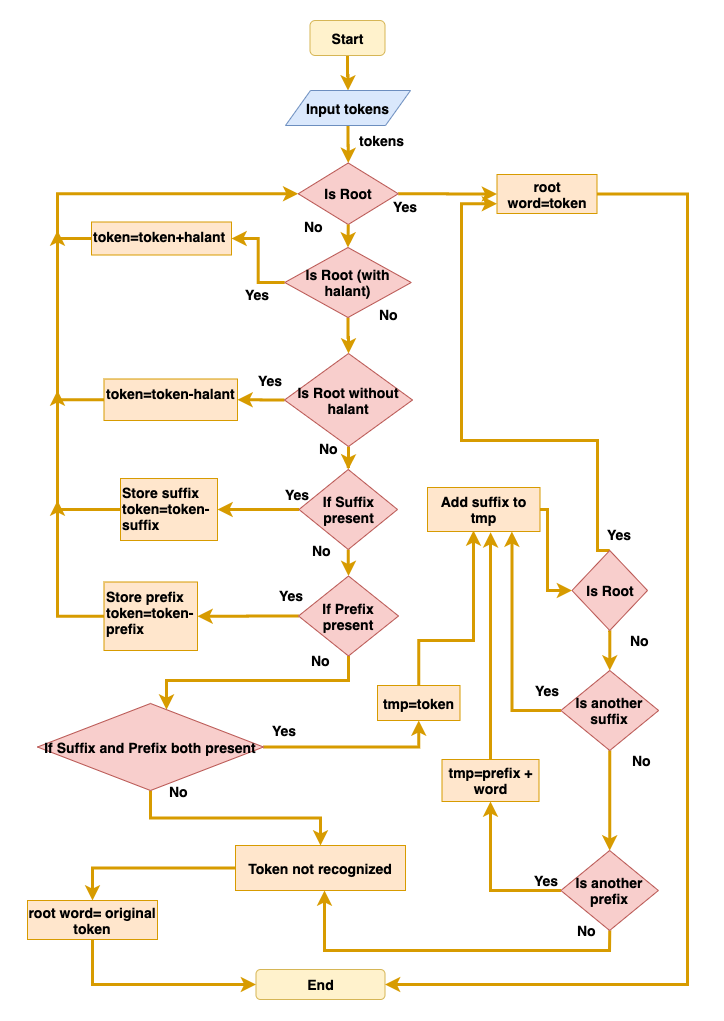
\includegraphics[width=0.8 \textwidth, keepaspectratio]{figures/stemming.png}
\caption{Detailed Flow diagram for stemming and lemmatization algorithm}
\label{stemming}
\end{figure}

\twocolumn

\item Inverse Document Frequency (idf)\\
     The inverse document frequency (idf) is the measure of how important a term
     is to the entire collection of documents in the corpus. It weighs down the
     effects of terms that occur too frequently while weighs up the effects of
     less frequently occurring terms by inverting the number of documents
     containing the particular term \cite{r6}. We calculate idf for each term
     which is mathematically given by (\ref{eq3})
\begin{equation}idf(t,D) = \ln\left({\frac{|D|}{|\{d\in D : t \in d\}|}}\right) \label{eq3}
\end{equation}
   \begin{gather*}
  \text{where},\\
  |D|=\text{Total number of documents in the corpus},\\
  |\{d\in D : t \in d\}| = \text{Number of documents}\\ \text{\qquad \qquad \quad \quad containing term t}
\end{gather*}
 \end{enumerate}

So, from (\ref{eq1}), (\ref{eq2}), and (\ref{eq3}), we can write the tf-idf as defined in (\ref {eq4})
\begin{equation}
tf\textnormal{-}idf= \frac{f_d(t)}{\sum_{w\in d}{f_d(w)}} \times \ln\left({\frac{|D|}{|\{d\in D : t \in d\}|}}\right) \label {eq4}
\end{equation}

An excellent example of how idf comes into play is for the word "the." 
We know that just about every document contains "the," so the term 
is not significant, thereby producing a very low IDF \cite{r7}. 
    
\subsection {Construction of vector (Vector Space Model)}
Using the relation in (\ref{eq4}), we construct tf-idf dictionaries for each
term-document pair. Thereupon, we create a matrix that consists of an array of
vectors, where each vector represents a document in the corpus. The vector will
be a list of frequencies for each unique word in the corpus -- the tf-idf value
if the word is in the document, or 0.0 otherwise. The set of documents in the
corpus is then viewed as a set of vectors in a vector space, as shown in Figure.~\ref{vector}.
Each term in the corpus will have its axis \cite{r8}.

\begin{figure}[htbp]
\centering
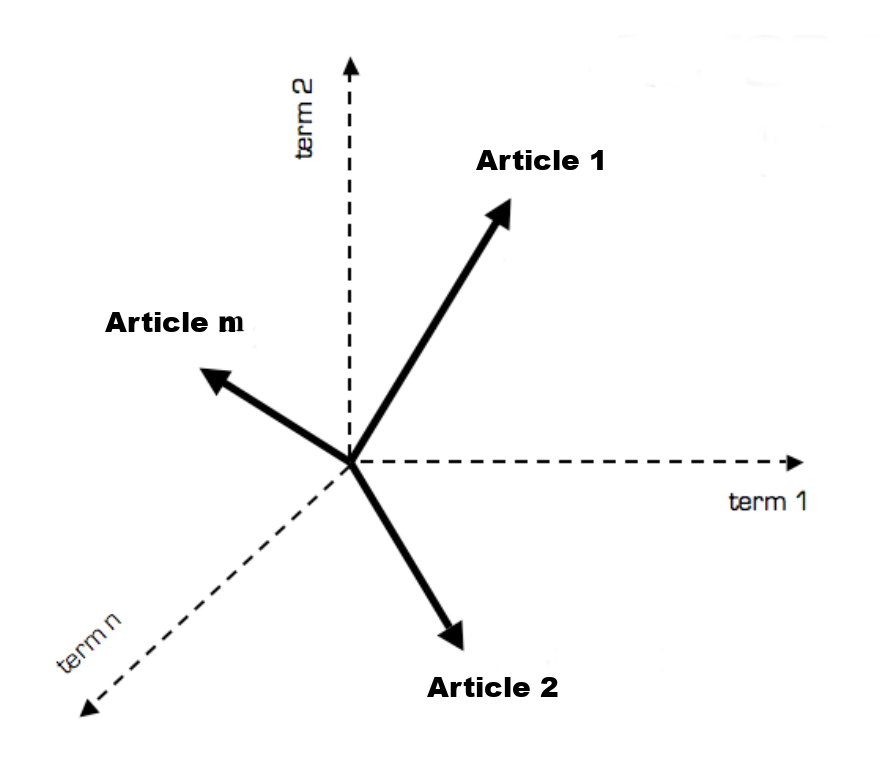
\includegraphics[width=0.4 \textwidth]{figures/vector.png}
\caption{Vector space model.}
\label{vector}
\end{figure}

\section{Calculating similarity}\label{AA}
\subsection {Cosine similarity}

It is a metric used to measure the degree of similarity between two
vectors. The vectors' size doesn't affect the similarity value since
the magnitude of the vectors automatically normalizes the value. We use
this metric to compute the similarity between pairs of news articles using the
equivalent tf-idf feature vector representation of the articles. Mathematically,
it measures the cosine of the angle between two vectors projected into a
multi-dimensional space. In this context, the two vectors are arrays containing
each term's tf-idf value in the two documents. 
\medskip

The cosine similarity is
advantageous because even if the two similar documents are far apart by the
Euclidean distance (due to the size of the document), chances are they may still
be oriented closer together. The smaller the angle, the higher, will be the
cosine similarity. When plotted on a multi-dimensional space, where each
dimension corresponds to a word in the document, the cosine similarity captures
the orientation (the angle) of the documents and not the magnitude \cite{r9}, as
shown in Figure.~\ref{cosine}. Using the formula given in (\ref{eq5}), we can
find out the cosine similarity between any two documents.

\begin{figure}[htbp]
\centering
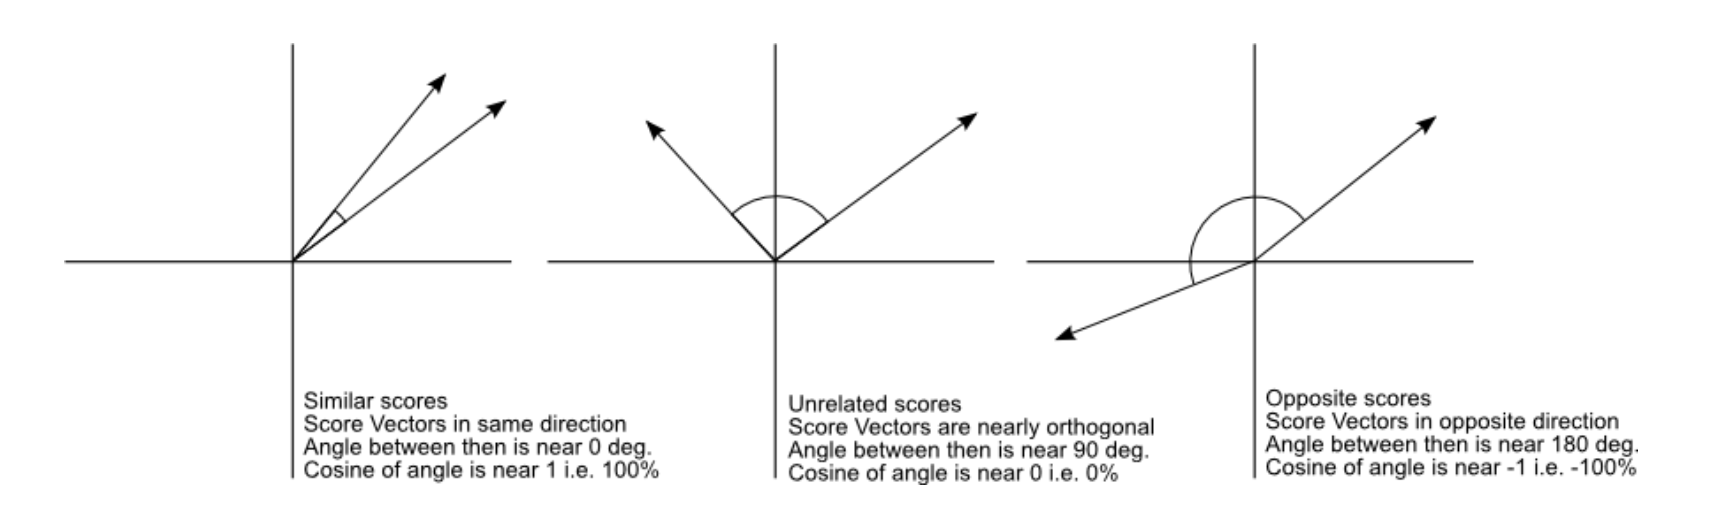
\includegraphics[width=0.5 \textwidth]{figures/cosine.png}
\caption{Cosine similarity visualization}
\label{cosine}
\end{figure}

\begin{equation}
\cos ({\vec a},{\vec b})= {{\vec a} . {\vec b} \over \|{\vec a}\| \|{\vec b}\|} = \frac{ \sum_{i=1}^{n}{{\vec a}_i{\vec b}_i} }{ \sqrt{\sum_{i=1}^{n}{({\vec a}_i)^2}} \sqrt{\sum_{i=1}^{n}{({\vec b}_i)^2}} } \label{eq5}
\end{equation}
 \begin{gather*}
  \text{where},\\
  \vec a \text{ and } \vec b \text{ represents tf-idf vectors of two documents},\\
  n \text{ is the length of the vector or vocabulary size}
\end{gather*}


\subsection {Jaccard similarity}
It is a measure to calculate the similarity between any two documents or terms
or sentences. To calculate the Jaccard similarity, the number of common
attributes is divided by the number of attributes in at least one of
the two objects. Jaccard Coefficient can also be used as a dissimilarity or
distance measure, unlike cosine similarity. If the Jaccard index between two
sets is 1, then the two sets have the same number of elements in the
intersection as the union, and we can show that ${A \cap B=A \cup B}$. So every
element in A and B is in A or B, so ${A = B}$. The Jaccard index can also be
used on strings. We define a set containing the characters in a
string for each string, so the string "cat" becomes {c, a,t}. If we have two strings, "catbird."
and "cat," then the numerator is 3, and the denominator is 7, which gives us a
Jaccard index of 3/7.

\begin{equation}
J(A,B) = \frac{|A\cap B|}{|A\cup B|}=\frac{|A\cap B|}{|A| + |B| -|A\cap B|}\label{eq6}
\end{equation}
\medskip

\section{Results and Discussions}

One of the major challenges in performing experiments for plagiarism detection
in Nepali texts was the lack of labeled datasets. We collected the following data
from different sources. These data have been made publicly
available\footnote{\url{https://github.com/ayushkumarshah/Nepali_Plagiarism_Detection/tree/master/datasets}}.

\subsection{Corpora}

\begin{enumerate}
\item NEP-PLAG2019v1\\
We collected 10000 pairs of Nepali news articles from different online news
portals sites and manually annotated them into plagiarised and non-plagiarised
pairs. This dataset is published as NEP-PLAG2019v1. It contains 4553 pairs 
of plagiarised and 5447 pairs of non-plagiarised articles. Hence, the classes
are almost balanced.
\medskip

\item Nepali root words\\
A total of 20,641 Nepali root words were collected from \href{http://ltk.org.np}{Language Technical Kendra}.
\medskip

\item Suffixes\\
A total of 135 Nepali suffixes were collected from \href{http://ltk.org.np}{Language Technical Kendra}.
\medskip

\item Prefixes\\
A total of 5 Nepali prefixes were collected from \href{http://ltk.org.np}{Language Technical Kendra}.
\medskip

\item Suffix and prefix rules\\
We wrote the rules for striping the corresponding suffixes and prefixes, respectively, to obtain root words.
\medskip

\item Stop words\\
A total of 592 stop words were collected from multiple online sources.

\end{enumerate}

\subsection{Experiment}

\begin{figure}[h!]
  \centerline{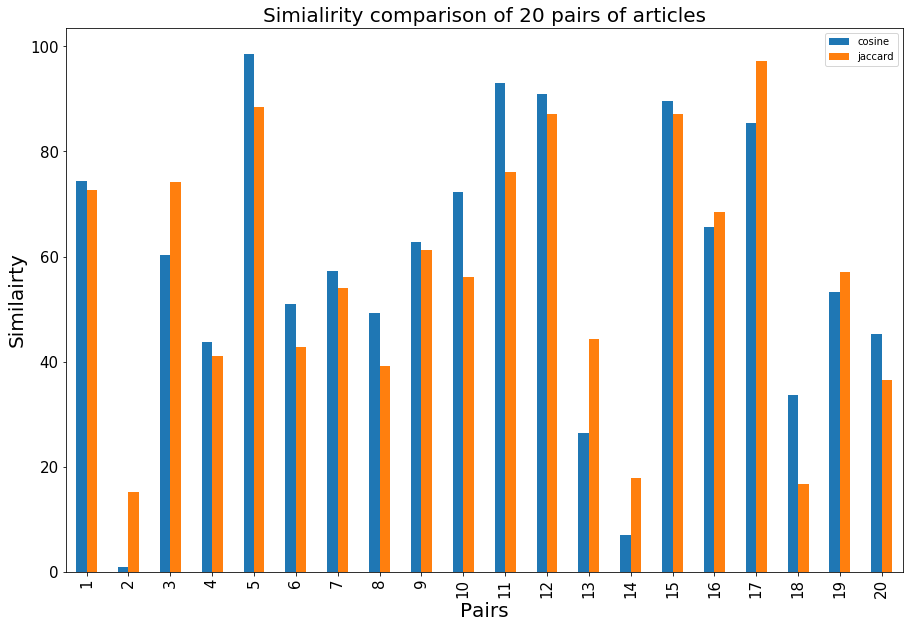
\includegraphics[width=0.4 \textwidth]{figures/similarity.png}}
\caption{Cosine and Jaccard similarity scores comparison for a random sample of 20 pairs of articles}
\label{similarity}
\end{figure}

For experimentation, we used the 10,000 pairs of annotated news articles in the
NEP-PLAG2019v1 dataset. We performed a rule-based recursive stemming algorithm on
the articles in the dataset using our rules to produce tokens consisting of 
the root words. We then fed the pre-processed tokens 
into the feature selection process to construct the tf-idf feature vectors as
per the process explained in the methodology section above. Both Cosine and
Jaccard similarity scores were computed for each pair of articles. The
comparison between the two score metrics in a random sample of 20 pairs of
articles from the corpus are shown in Figure.~\ref{similarity}.

Unlike the Cosine similarity score, the Jaccard similarity does not take the 
frequency of input tokens into account. Also, the comparison of results obtained 
from Cosine similarity and Jaccard similarity for
all the articles' pairs confirm that Cosine similarity always yields
better results. Hence, we use only the Cosine similarity score for
classification of article pairs. 

\begin{table}[htbp]
\caption{Confusion matrix on classification of 10,000 pairs of news articles
in the NEP-PLAG2019v1 dataset}
\begin{center}
\begin{tabular}{cc|cc}
\multicolumn{2}{c}{}
&\multicolumn{2}{c}{\textbf{Predicted}} \\
& & \textbf{Plagiarised} & \textbf{Non-plagiarised}\\ 
\cline{2-4}
\multirow{2}{*}{\rotatebox[origin=c]{90}{\textbf{Actual}}}
    & \textbf{Plagiarised}   & 4397   & 156                 \\
    & \textbf{Non-plagiarised}  & 205  & 5242                \\ 
    \cline{2-4}
    \end{tabular}
\label{conf}
\end{center}
\end{table}

\begin{table}[h!]
\caption{Evaluation Metrics on classification of 10,000 pairs of news articles
in the NEP-PLAG2019v1 dataset}
\begin{center}
\begin{tabular}{|c|c|}
\hline
\textbf{Evaluation Metrics}&{\textbf{Value}} \\
\hline
Accuracy & 96.39\%\\
Precision & 95.54\%\\
Recall & 96.57\%\\
F1-Score & 96.05\%\\
\hline
 \end{tabular}
\label{eval}
\end{center}
\end{table}

A threshold of 25\% cosine similarity score was used to classify 
each pair of articles as plagiarised or
non-plagiarised. The confusion matrix obtained in the classification task on
10,000 pairs of articles in the NEP-PLAG2019v1 dataset is shown in 
Table \ref{conf}. Also, the results of the evaluation metrics on the same 
task are shown in Table \ref{eval}.

\subsection{Discussions and Comparisons}
Rule-based segmentation approaches have been used in Devanagari scripts in previous works
\cite{abhishek_effective_2013} as well. However, most of the rule-based and
other previous approaches \cite{dangui_lightweight_2015, pande_devanagari_nodate}
have not considered the complex grammatical rules specific to Nepali language
and the dependency of the stemming and lemmatization behaviour on the POS of the
derived word in the sentence. Moreover, \cite{dangui_lightweight_2015} does not
consider prefixes for extracting the root word, and hence returns invalid root
words for words containing prefixes. The use of lookup tables is not efficient
in terms of computation and time as well. Also, the approaches generalized for many
languages based on the Devanagari script 
\cite{dangui_lightweight_2015, pande_devanagari_nodate} fails to capture the
unique changes in the vowels and consonants of a specific language, here Nepal
texts, during the inflection of derived words into the root words. These factors
contribute to a decrease in the accuracy of obtaining a valid root word,
ultimately affecting the plagiarism classification. 

The proposed method has tackled with these limitations by defining both prefix
and suffix rules, which are applied recursively until the root word is obtained.
The approach can 
handle any unique cases of changes in the vowel or consonant, specific to
Nepali texts as well. Likewise,
including the POS tags in the rule adds the ability to apply different rules to
the words with consideration to the POS of the word in the sentence.
Improvements have been made to ensure that the root word is almost always valid
by using a dictionary to perform lemmatization.

For feature selection, tf-idf feature vectors are used, since they are easy to
compute and represent the texts well. They give fair results for plagiarism
tasks since the dataset used was relatively simple. However, tf-idf feature
vector is likely to fail in capturing the features of a complex dataset since it
cannot capture the semantic context in the sentence and document level. Hence,
for future works, tf-idf should be replaced by other complex embedding models like
word2vec or BERT.

The results obtained from the task of plagiarism detection using the proposed 
rule-based recursive segmentation and tf-idf feature vector construction with
Cosine similarity have been compared with approaches using
previous methods of stemming and pre-processing but with the same
post-processing steps using tf-idf and Cosine similarity on the NEP-PLAG2019v1 dataset 
in the Table \ref{comparison}.

\begin{table}[htbp]
\caption{Comparison of Plagiarism classification F1-scores on 10,000 pairs of
articles in the NEP-PLAG2019v1 dataset}
\begin{center}
\begin{tabular}{|c|c|}
\hline
\textbf{Method} & {\textbf{F1-score}} \\
\hline
Rule-based recursive lemmatization$^*$ & 96.05\% $^*$\\
\hline
Effective Devanagari Hindi Stemmer \cite{abhishek_effective_2013} & 86.05\% \\
\hline
Lightweight general Devanagari Stemmer\\ using n-gram \cite{dangui_lightweight_2015} & 87.05\% \\
\hline
Romanization based stemmer \cite{pande_devanagari_nodate}& 92.05\% \\
\hline
\end{tabular}
\label{comparison}
\end{center}
\end{table}

The comparison results clearly show that the proposed method outperforms the
previous stemmers designed for Devanagari scripts.

\section{Conclusion}

The paper introduced a stemming algorithm using a set of custom-defined
recursive rules to pre-process Devanagari
scripts specifically for the Nepali language, considering the complex syntactic
and grammatical structures, and dependency on POS of the word in order to 
detect plagiarism with higher F1-score in Nepali articles. Since the proposed
algorithm is able to outperform previous Devanagri script-based stemmers, 
it can be a helpful step in various NLP tasks in Nepali texts, other than Plagiarism as
well. Most of the NLP tasks include the pre-processing step before 
employing the main algorithm or the
required task. Moreover, this algorithm can be extended to other languages as
well by developing similar recursive rules as per the grammatical rules of the
corresponding language and incorporating the variation in the rules to
represent POS dependency. Hence, this paper has a wide range of applications in
the field of NLP. 

The obvious limitation to this approach is the algorithm's non-robust nature 
since the grammatical and syntactic rules required in this algorithm need to be
defined manually, which is dependent on the language completely. Likewise, the
semantic and contextual information in the texts is not considered, which may 
reduce the performance in a large dataset. Due
to insufficient dataset of Nepali texts, the evaluations performed in this 
paper were done on our own NEP-PLAG2019v1 dataset. Hence, the evaluation may 
not be a standard benchmark for comparing the performance.

In the future, we plan to overcome the current limitation by incorporating semantic
and contextual information during the computation of the similarity measures by
using deep learning approaches to capture the context of the words instead of
relying on the frequency entirely. Likewise, another approach may be 
comparing the similarities of the obtained
tokens' meanings by constructing and using a dictionary instead of the similarities
between the tokens. Thereby, we need to construct a corpus containing Nepali
root words and their corresponding meanings. When similarity is measured at a
semantic level, sentences having different words but giving the same meaning
will get a higher similarity score.

\section*{Acknowledgment}
Our thanks to our supervisor, Associate Professor Bal Krishna Bal,
for assisting and guiding us throughout the project and sincere thanks to 
\href{http://ltk.org.np/}{Language Technical Kendra} for providing us the
required datasets and resources.

\bibliographystyle{IEEEtran} 
\bibliography{references}

\end{document}
